The development of this notation will largely follow \cite{brown2010efficient}.

Let $\lbrace X_i \rbrace_{i = 1}^P$ denote the Legendre-Gauss-Lobatto (LGL) nodes of degree $P - 1$ on the reference interval $\left[ -1, 1 \right]$ while $\lbrace q_i \rbrace_{i = 1}^Q$ and $\lbrace w_i \rbrace_{i = 1}^Q$ denote the quadrature points and quadrature weights corresponding to a $Q$ point quadrature rule.
If we consider Lagrange basis functions $\lbrace \phi_i \rbrace_{i = 1}^P$, we can construct matrices $B_{i j} = \phi_j \left( q_i \right)$, $D_{i j} = \partial_x \phi_j \left( q_i \right)$, and $W_{i j} = w_i \delta_{i j}$, representing interpolation to the quadrature points, computation of derivatives at the quadrature points, and quadrature weights, respectively.

We can define the corresponding matrices for 3D problems via tensor products
\begin{equation}
\begin{array}{c}
\mathbf{B}   = B \otimes B \otimes B \hspace{5mm}
\mathbf{D}_0 = D \otimes B \otimes B\\
\mathbf{D}_1 = B \otimes D \otimes B \hspace{5mm}
\mathbf{D}_2 = B \otimes B \otimes D\\
\mathbf{W}   = W \otimes W \otimes W
\end{array}
\label{basis_ops}
\end{equation}
The basis operations \ref{basis_ops} are defined on a reference element $\hat{K} = \left[ -1, 1 \right]^3$.
In the finite element and spectral element methods, we partition the domain $\Omega$ into a set of $E$ elements, denoted $\lbrace K^e \rbrace_{e = 1}^E$ with coordinate mapping to the reference element given by $X : \hat{K} \rightarrow K^e$.
The Jacobian of this mapping is given by $J_{i j} = \partial x_i / \partial X_j$, where $X$ is the reference coordinates and $x$ the physical coordinates.
We can invert the Jacobian and compute the derivatives of the physical coordinates in the reference space at every quadrature point.
\begin{equation}
\mathbf{D}_i^e = \Lambda \left( \frac{\partial X_0}{\partial x_i} \right) \mathbf{D}_0 + \Lambda \left( \frac{\partial X_1}{\partial x_i} \right) \mathbf{D}_1 + \Lambda \left( \frac{\partial X_2}{\partial x_i} \right) \mathbf{D}_2
\end{equation}
where $\Lambda \left( X \right)_{i j} = X_i \delta_{i j}$ expresses pointwise multiplication of $J_{i j}^{-1}$ at quadrature points as a diagonal matrix.
With this coordinate mapping, element integration weights become $\mathbf{W}^e = W \Lambda \left( \lvert J^e \left( q \right) \rvert \right)$.

When using an assembled matrix to represent a finite element operator, a global assembly operator is defined as $\mathcal{E} = \left[ \mathcal{E}^e \right]$, where $\mathcal{E}^e$ represents local restriction operators extracting degrees of freedom that correspond to element $e$ from the global solution vector.
Notice that these local restriction operators do not assume a structured mesh, a conforming mesh, or consistent polynomial order bases for each element.

With these definitions, we can represent the Galerkin system of equations corresponding to the weak form of arbitrary second order PDEs.
The weak form of PDEs is linear in test functions and can be expressed as pointwise operations where functions of $u$ and $\nabla u$ are contracted with $v$ and $\nabla v$.

Consider the weak form of an arbitrary PDE
\begin{equation}
\begin{array}{c}
\text{find } u \in V \text{ such that for all } v \in V\\
\langle v, u \rangle = \int_{\Omega} v \cdot f_0 \left( u, \nabla u \right) + \nabla v : f_1 \left( u, \nabla u \right) = 0
\end{array}
\label{weak_form}
\end{equation}
where $\cdot$ represents contraction over fields and $:$ represents contraction over fields and spatial dimensions.
The pointwise representation of the weak form given by $f_0$ and $f_1$ does not depend upon discretization choices such as geometry or polynomial degree of the bases.
The corresponding Galerkin system of equations is
\begin{equation}
\sum_e \mathcal{E}^T \left[ \left( \mathbf{B}^e \right)^T \mathbf{W}^e \Lambda \left( f_0 \left( u^e, \nabla u^e \right) \right) + \sum_{i = 0}^{d - 1} \left( \mathbf{D}_i^e \right)^T \mathbf{W}^e \Lambda \left( f_1 \left( u^e, \nabla u^e \right) \right) \right] = 0
\label{galerkin_form}
\end{equation}
where $u^e = \mathbf{B}^e \mathcal{E}^e u$ and $\nabla u^e = \lbrace \mathbf{D}_i^e \mathcal{E}^e u \rbrace_{i = 0}^{d - 1}$.
In this formulation, the element restriction operators and basis operators can represent different element geometries and different degree polynomial bases, providing a flexible description for arbitrary meshes.
Furthermore, this notation can be extended to handle separate fields with different bases, such as with mixed finite element methods.

Dirichlet boundary conditions are represented in the element restriction operation by enforcing the specified values on the constrained nodes.
Neumann or Robin boundary conditions are represented by adding boundary integral terms in the same form as \ref{galerkin_form} with appropriate basis and element restriction operators.
Boundary integrals internal to the domain $\Omega$, such as face integrals in Discontinuous Galerkin methods, can also be represented using additional terms with corresponding bases and element restrictions.

% -- Linearization -------------------------------------------------------------
\subsection{Linearization}

% NOTE: Figure moved in the source to overcome some LaTeX positioning stupidity
\begin{figure}
\begin{subfigure}{.495\textwidth}
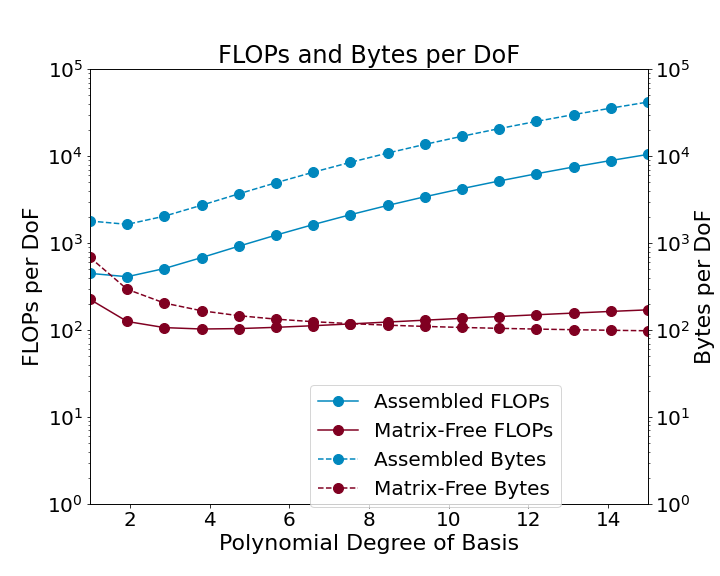
\includegraphics[width=.99\linewidth]{../img/assembledVsMatrixFree}
\caption{FLOPs and Bytes per DoF}
\end{subfigure}
\begin{subfigure}{.495\textwidth}
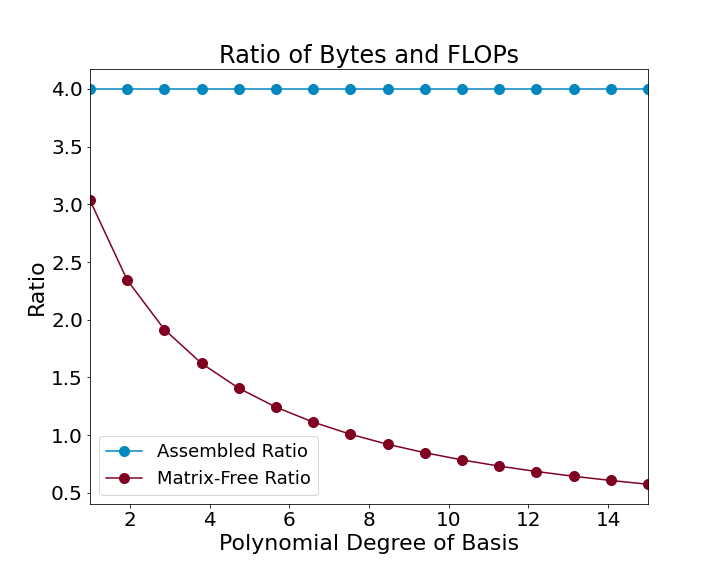
\includegraphics[width=.99\linewidth]{../img/assembledVsMatrixFreeBalance}
\caption{Ratio of Bytes to FLOPs}
\end{subfigure}
\caption{Performance per DoF}
\label{fig:assembledvsmatrixfree}
\end{figure}

When the PDE \ref{weak_form} is linear, the pointwise functions $f_0$ and $f_1$ are also linear and Krylov subspace methods can be used to solve the Galerkin system of equations \ref{galerkin_form}.
When the PDE is non-linear, the Galerkin system \ref{galerkin_form} provides the residual evaluator for a non-linear solver and Jacobian can be represented in a similar fashion as \ref{galerkin_form}, based upon the weak form
\begin{equation}
\langle v, J \left( u \right) w \rangle = \int_{\Omega}
\left[ \begin{array}{c c}
v^T & \left( \nabla v \right)^T
\end{array} \right]
\left[ \begin{array}{c c}
f_{0, 0} & f_{0, 1}\\
f_{1, 0} & f_{1, 1}
\end{array} \right]
\left[ \begin{array}{c c}
w & \nabla w
\end{array} \right]
\label{jacobian_form}
\end{equation}
where $f_{i, 0} = \frac{\partial f_i}{\partial u} \left( u, \nabla u \right)$ and $f_{i, 1} = \frac{\partial f_i}{\partial \nabla u} \left( u, \nabla u \right)$.
If these pointwise functions $f_{i, j}$ are not available analytically, they can be computed via algorithmic differentiation or finite differencing.

With these pointwise functions, we can describe Jacobian-free Newton-Krylov methods for solving non-linear PDEs.
Jacobian-free Newton-Krylov methods were summarized, with preconditioning strategies, by Knoll and Keyes in \cite{knoll2004jacobian}.

% -- Performance ---------------------------------------------------------------
\subsection{Performance}

To demonstrate the performance benefits of high-order finite elements implemented in a matrix-free fashion, we consider the specific case of the screened Poisson equation, $\nabla^2 u - \alpha^2 u = f$.
In this case, application of the finite element operator for a single element requires $\mathcal{O} \left( P^6 \right)$ matrix entries and $\mathcal{O} \left( P^6 \right)$ floating point operations.
In contrast, application of the matrix-free operator for a single element requires $\mathcal{O} \left( P^3 \right)$ floating point values and $\mathcal{O} \left( P^{d + 1} \right)$ floating point operations.

As seen in Figure \ref{fig:assembledvsmatrixfree}, the balance between bandwidth and FLOPs for matrix-free implementations more closely agrees with current HPC hardware capabilities.

In comparison to the generation of simplex meshes, generation of high quality hexahedral meshes is a time intensive process.
However, it is possible to generate meshes comprised predominately of high quality hexahedral elements with initial refinement of a simplex mesh without the costly process of fully converting a simplex mesh into hexahedral elements.
Thus, the performance benefits of high-order matrix-free finite elements can be realized without substantial additional effort in generating a mesh exclusively composed of high quality hexahedral elements.
